
\chapter{SLAM基础}
\section{闭环检测}
没有闭环检测的SLAM系统叫做视觉里程计(VO),视觉里程计随着时间的推移,误差会随之累计,从而导致位姿误差累计,从而导致3D点位置的不正确,从而导致在闭环处,本应该相同的3D场景点,被重建到了不同的3D点,并且离得还挺远的,从而导致了漂移。如下图所示:

\begin{figure}[h]%%图
	\centering  %插入的图片居中表示
	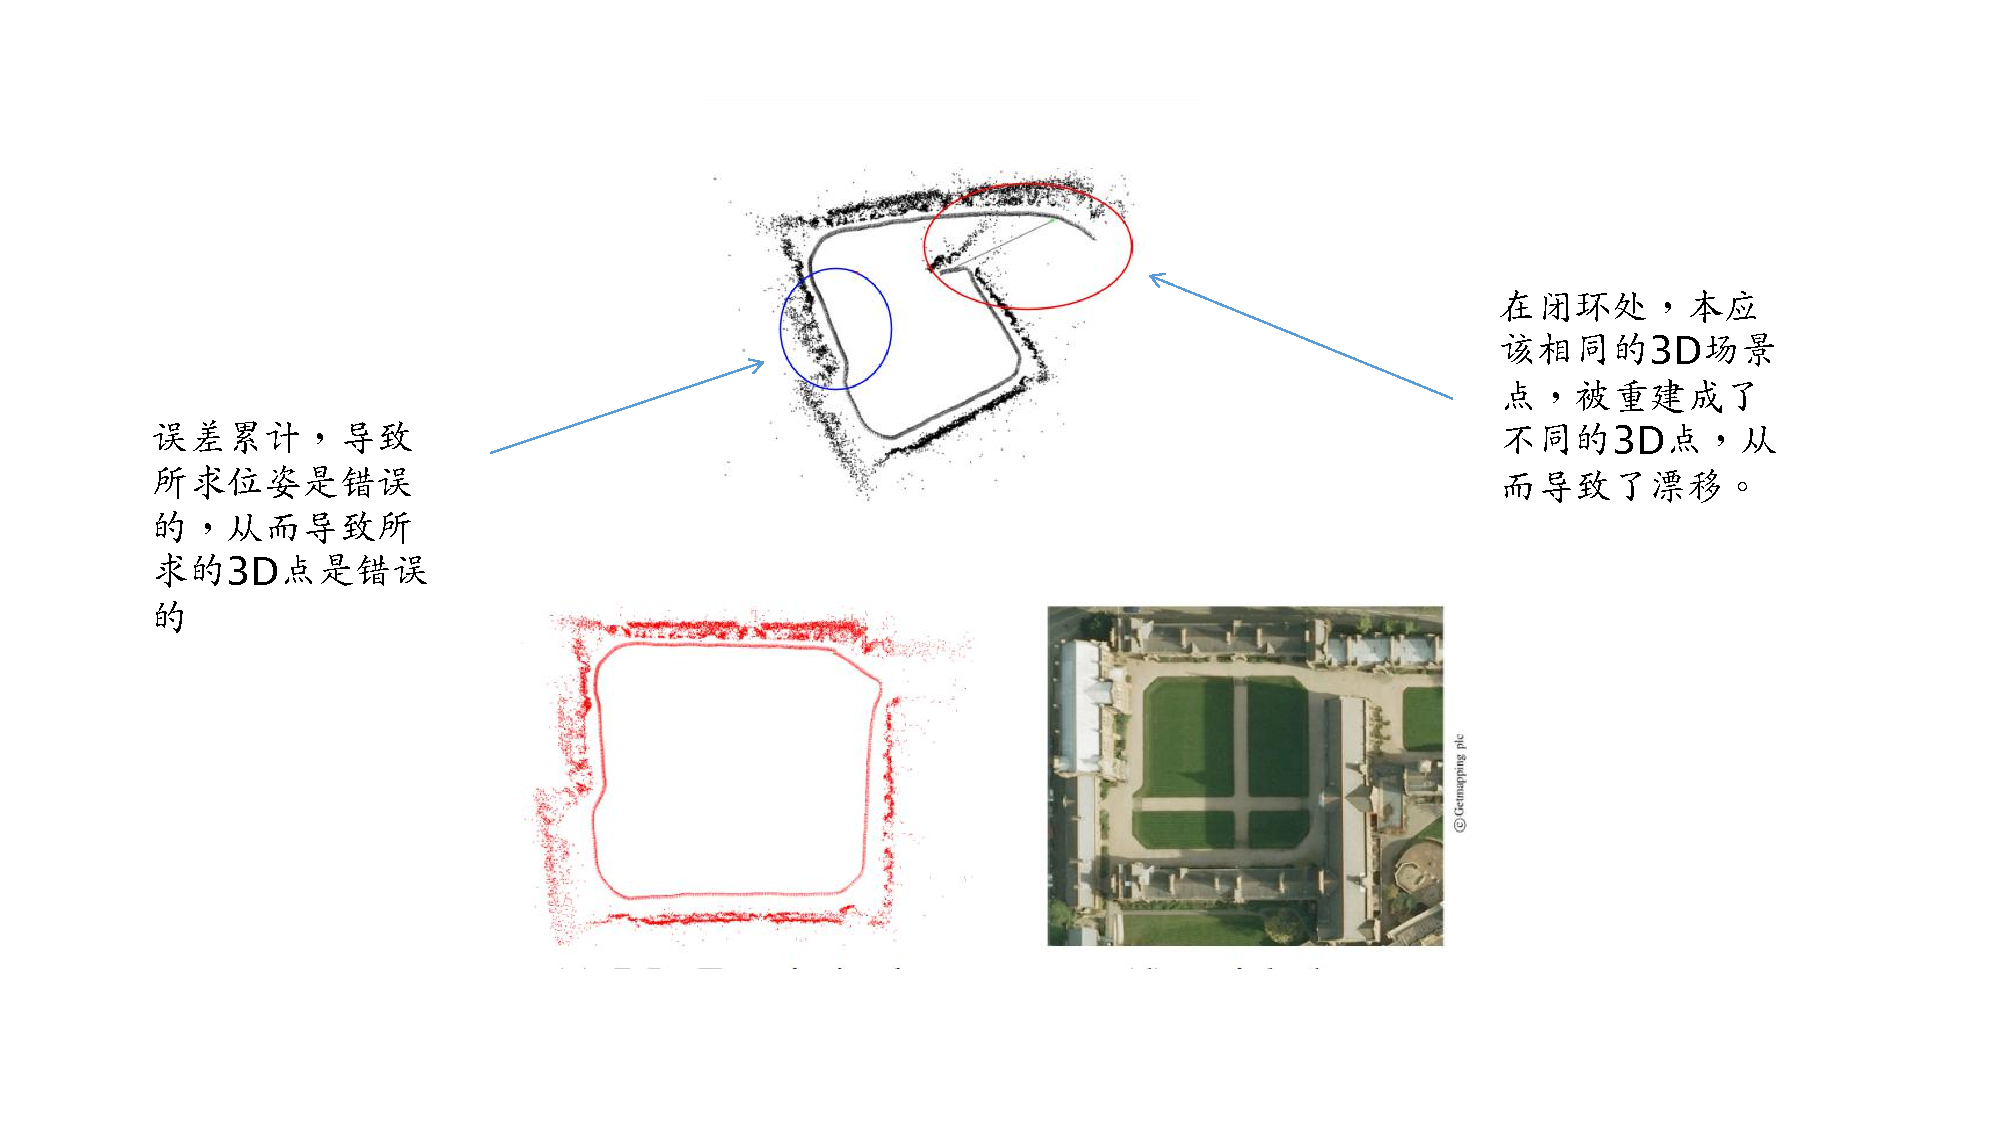
\includegraphics[width=1.0\linewidth]{image/drift.pdf}  %插入的图,包括JPG,PNG,PDF,EPS等,放在源文件目录下
	\caption{3D点误差累积及漂移.}  %图片的名称
	\label{fig:tracking}   %标签,用作引用
\end{figure}


相机的位姿不准(累积误差),从而导致3D点的位置不准,在闭环处就表现为:\textbf{本应该重合的3D点,因为位姿不准,而不重合了,漂移了},我能理解漂移,但是不能够理解\textbf{尺度漂移}。

而\textbf{闭环纠正},就是使用很久之前很久之前的相机位姿(准)重新计算闭环的相机位姿(不准->准),从而减少了累积误差,但是这里的重新计算只是纠正了闭环帧的累积误差,为了进一步减少其它帧的累积误差,我们需要将结果传播出去,具体表示为pose graph优化,但是pose graph优化又认为相对位姿是准的,这就令我很不明白了。




\textbf{pose graph的约束都是如何得到的}:
\begin{enumerate}
	\item 相邻关键帧之间的位姿约束
	\item 时间序列上比较接近的关键帧之间的位姿约束(可以称作局部回环),比如t时刻的关键帧不仅仅与t-1时刻的关键帧构成约束关系,还会与t-2时刻的关键帧构成约束关系。
	\item  时间序列上不接近,而空间上接近的关键帧之间的位状约束(可以称作大回环),一般来说,机器人绕着房子周围走了一圈回到了起点,那么检测到的回环就是大回环。
\end{enumerate}





\section{Pose Graph和闭环检测}
带有相机位姿和空间点的图优化称为 BA,能够有效地求解大规模的定位与建图问题。BA能够有效解决漂移(从我实现SFM系统的经验可得),但是由于BA数据量太大了,不适合需要实时性的SLAM。适合SLAM优化的解决方案有两种,一种是移动窗口BA;另一种就是Pose Graph。
	
Pose Graph就是将相机的绝对位姿作为图的结点(待优化变量),而相机之间的相对位姿作为边(约束条件),当遇到回环时,通过位姿图进行优化,就能够减少累计误差。

\begin{note}
	不是很理解位姿图优化,不会将位姿优化飘掉吗?
\end{note}
	
使用frame-to-frame的方式求得的位姿,会使得误差逐渐累积,从而导致位姿越来越不准。因为后一帧图像的位姿是基于前一帧图像进行计算的,如果前一帧图像的位姿具有误差,哪怕很小,那么后一帧图像计算得到的位姿也会使得误差增加。随着SLAM系统的不断运行,这个误差就越来越大,从而导致相机都轨迹都出现了漂移。

\begin{figure}[h]%%图
	\centering  %插入的图片居中表示
	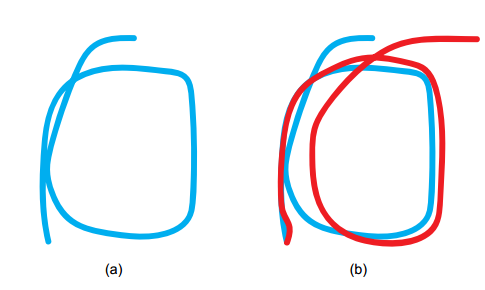
\includegraphics[width=0.7\linewidth]{image/Trajectory_drift}  %插入的图,包括JPG,PNG,PDF,EPS等,放在源文件目录下
	\caption{漂移示意图。( a)真实轨迹;( b)漂移轨迹.}  %图片的名称
	\label{fig:Trajectory_drift}   %标签,用作引用
\end{figure}
	
虽然随着SLAM系统的运行,相机的绝对位姿的误差会越来越大,但是相邻两关键帧之间的位姿还是挺准确的,所以每个关键帧和其前续(predecessor)关键帧之间的相对位姿可以构成一个约束。

\begin{note}
	相邻关键帧的位姿态就一定准确吗?对于RGB-D相机,计算相邻关键帧的位姿时,使用的3D点是从相机得到的,那么计算得到的相邻位姿应该是准确的;但是对于RGB相机,使用的3D点就是具有累计误差的,那么使用该3D点计算得到的相邻位姿应该不能认为是准确的吧。
\end{note}
